\chapter{Drupal} \label{Drupal}

\section{Wat is Drupal?}

\begin{wrapfigure}{r}{0.3\textwidth}
\vspace{-40pt}
%\hspace{-10pt}
\centering
\label{fig:drupalLogo}

\includegraphics[width=0.3\textwidth]{fig/drupalLogo}
\vspace{-30pt}
%\hspace{-10pt}
\centering
\caption{Drupallogo}
\centering
\vspace{-40pt}
\end{wrapfigure}
We kunnen Drupal het best beschrijven aan de hand van Figuur~\ref{fig:watIsDrupal}.
Drupal is een Content Management System (CMS)\nomenclature{CMS}{Content Management System}, een framework voor webapplicaties en een social publishing platform. Maar Drupal is meer dan software alleen. Drupal staat voor een gemeenschap van ontwikkelaars en gebruikers met uiteenlopende doeleinden die elk hun eigen visie willen realiseren. \cite{drupalDefGuide}

\subsubsection{Content Management System}

Drupal levert alle functies en mogelijkheden van een krachtig CMS. We denken meteen aan het kunnen inloggen en registreren van gebruikers, verschillende soorten gebruikers kunnen defini\"{e}ren, verschillende niveaus van permissies,... Ook denken we aan het cre\"{e}ren, aanpassen, beheren, weergeven, categoriseren en aggregeren van content. Drupal biedt bovendien de mogelijkheid om modulair extra functionaliteit toe te voegen naar eigen noden en wensen.

\subsubsection{Framework voor webapplicaties}

Drupal is enorm flexibel en krachtig waardoor er enorm veel verschillende soorten webapplicaties mee kunnen gebouwd worden. Dit is deels te danken aan de API's die Drupal aanbiedt. Deze worden bij elke versie van Drupal uitgebreid maar ze worden niet complexer om te gebruiken. Drupal's veelzijdigheid wordt nogmaals bewezen met het feit dat het zowel als frontend voor Java-gebaseerde applicaties kan optreden of als backend voor AJAX of Flash-driven frontends.

\subsubsection{Social publishing platform}

Dat Drupal een social publishing platform is, houdt in dat content gemakkelijk te delen is via Drupal. Drupal biedt de mogelijkheid complexe data in een structuur te gieten welke gemakkelijk uit te wisselen is. Op deze manier is het gemakkelijk eenzelfde stuk data voor te stellen op verschillende websites.

\begin{figure}[h]
\centering
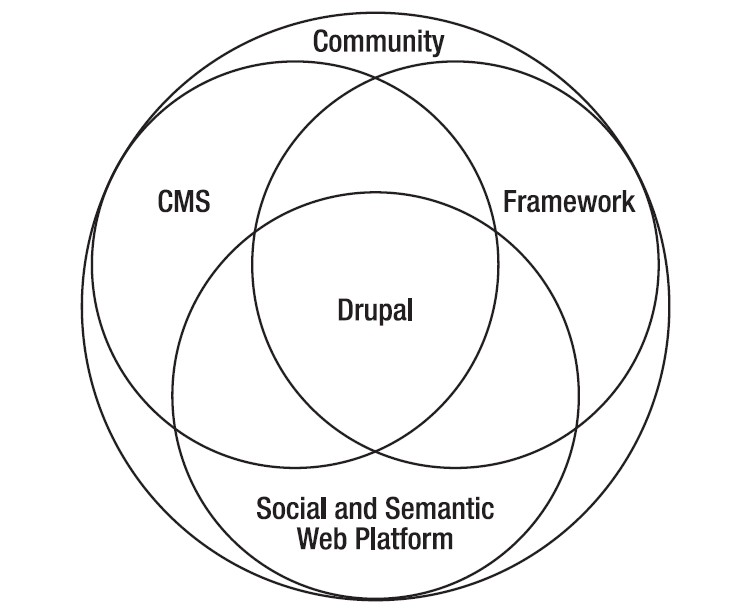
\includegraphics[width=0.4\textwidth]{fig/watIsDrupal}
\caption{Wat is Drupal?}
\vspace{-10pt}
\label{fig:watIsDrupal}
\end{figure}

We kunnen Drupal ook beschrijven als een gratis softwarepakket dat je de mogelijkheid biedt om jouw inhoud gebruiksvriendelijk te beheren en te publiceren. En dit op zo een manier dat je een eindeloze graad van personalisering hebt. Deze inhoud kan bestaan uit allerlei dingen, zoals: een blog, een video, een foto, een artikel, resultaten van een experiment,... Algemeen is dit dus een combinatie van tekst, beelden en audio die bezoekers van je website kunnen zien, lezen en/of horen. Bovendien is Drupal open source.

Drupal is ontwikkeld in PHP en gebruikt ook een noemenswaardige hoeveelheid JavaScript (in de vorm van jQuery) voor de frontend. Voor het opslaan van content en configuratiegegevens gebruikt Drupal een relationele databank. Drupal in zijn huidige versie (7) kan op elk platform draaien onder volgende twee voorwaarden:
\begin{itemize}
\item Het platform bevat een webserver die PHP, en dus server-side scripting ondersteunt. Voorbeelden van deze webserver zijn:  Apache, IIS, Lighttpd en nginx.
\item Het platform ondersteunt een van volgende databanktechnologie\"{e}n: MySQL, SQLite of PostgreSQL.
\end{itemize}
Bij deze masterproef wordt er gebruik gemaakt van Apache en MySQL.

\subsection{Basiswebsite}

Wanneer je Drupal installeert beschik je meteen over een basiswebsite. Omdat je meteen al een bruikbare website hebt, is de drempel om Drupal te beginnen gebruiken dus laag. Deze website biedt meteen al een heleboel functionaliteit aan die geleverd wordt door de zogenaamde Drupal Core en een aantal out-of-the-box functies.
\begin{figure}[h]
\begin{center}
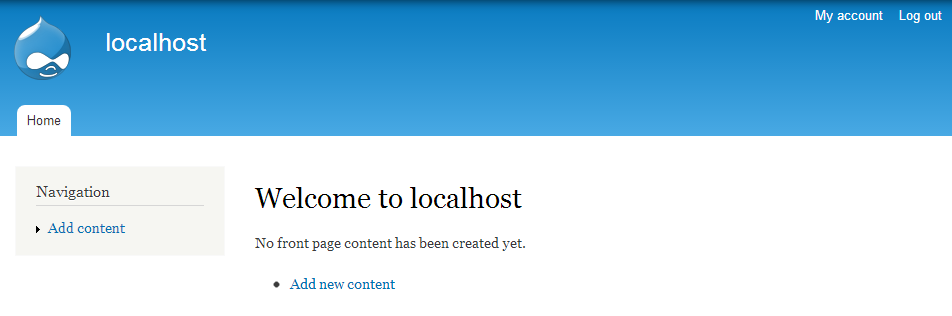
\includegraphics[keepaspectratio,width=1\textwidth]{fig/drupalBasiswebsite}
\vspace{-30pt}
\caption{Basiswebsite van Drupal met Bartik-theme}
\vspace{-30pt}
\end{center}
\end{figure}

\section{Waarom Drupal?}

Eerst sommen we de vlakken op waar elke degelijke software goed op moet scoren:
\begin{itemize}
\item betrouwbaarheid en robuustheid
\item effici\"{e}ntie
\item flexibiliteit
\end{itemize}
Als we dit even vergelijken met de principes waarop Drupal gebouwd is:
\begin{itemize}
\item Modulair en uitbreidbaar: Drupal kan uitgebreid worden met modules, waarbij je zelf ook modules kan ontwerpen indien er nog geen bestaat die aan jouw noden voldoet. Dit draagt dus bij aan de flexibiliteit.
\item Kwaliteitsvolle codering: kwaliteitsvolle, elegante en goed gedocumenteerde code is een prioriteit. Dit draagt bij tot de robuustheid en betrouwbaarheid.
\item Standard-based: Drupal maakt gebruik van ingeburgerde standaarden zoals bvb. XHTML en CSS. Dit draagt ook bij tot de robuustheid en betrouwbaarheid.
\item Low-resource demanding: om een goede prestatie te garanderen, maakt Drupal gebruik van low-profile codering (bvb. minimaliseren van databasequeries). Dit draagt bij tot de effici\"{e}ntie.
\item Open source: Drupal is gebouwd op en kan gebruikt worden in andere open source projecten.
\item Gebruiksvriendelijk: Drupal moet gemakkelijk te gebruiken zijn, zowel voor gebruikers, ontwikkelaars en administrators van een website.
\item Samenwerking: Drupal voorziet systemen om samenwerking te bevorderen, waaronder het versiebeheersysteem GIT.
\end{itemize}
We zien dat Drupal aan de eerder vermelde voorwaarden voldoet.\\

Een bijkomend voordeel van Drupal is zijn grote gemeenschap die ondertussen uit al meer dan 630000 actieve gebruikers en ontwerpers bestaat die zich dagelijks inspannen om Drupal steeds beter te maken. Dit aantal neemt elke dag toe. Dankzij die grote gemeenschap krijg je snel antwoord op je vragen door de medewerking van andere Drupal leden.\\

We bespreken nu enkele nadelen van Drupal:
\begin{itemize}
\item Aangezien Drupal gebruik maakt van een databank, heb je een databankserver nodig, al dan niet op dezelfde fysieke server als de webserver.
\item Bovendien wordt telkens een pagina wordt opgevraagd, de bootstrapcode uitgevoerd, waarbij ook nog eens de databank veelvuldig wordt geraadpleegd. 
Dit maakt Drupal relatief traag.
\item Drupal is zeer gebruiksvriendelijk en ideaal voor de eindgebruikers, die gemakkelijk en interactief inhoud willen toevoegen en beheren. 
Beginnende Drupal-ontwikkelaars zullen evenwel merken dat Drupal een erg steile leercurve heeft.
\item Ook ben je afhankelijk van de Drupal-community en dus de goodwill van de andere leden. Dit is in veel gevallen een voordeel, maar wanneer je een probleem hebt, ben je niet zeker of er wel een oplossing voor bestaat.
\item Tenslotte kan iedereen een module maken. Dit heeft natuurlijk zijn voordelen maar wanneer je een module van iemand anders gebruikt, ben je nooit zeker of de module zal onderhouden worden naar de toekomst toe en of er al dan niet bugs in zitten.
\end{itemize}

\section{Werking van Drupal}

Aan de hand van een voorbeeld \cite{drupalDefGuide} proberen we de lezer een idee te geven van de werking van Drupal. Bekijk Drupal als een digitale postzegelsorteerder. De nodes zijn de postzegels en de content types zijn de verschillende soorten postzegels (postzegels van \euro~0,67, \euro~1,34, ... ). Naast content types, kan je taxonomy gebruiken om een verdere onderverdeling te maken in de postzegels. De mate waarin en de criteria waarop je je onderverdeling maakt, kan je zelf kiezen (land, kleur, ...). Views is het mechanisme dat je postzegels sorteert en weergeeft in de vorm van pagina's en blocks. Van deze pagina's en blocks kan je zelf grootte, vorm, kleur en andere criteria opstellen zodat je deze helemaal kan personaliseren. Zie Figuur~\ref{fig:drupalGrafischeWeergave}.

\begin{figure}[h]
\centering
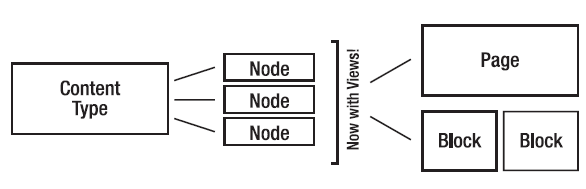
\includegraphics{fig/drupalGrafischeWeergave}
\centering
\vspace{-10pt}
\caption{Grafische weergave van hoe Drupal content aanbiedt.}
\vspace{-10pt}
\label{fig:drupalGrafischeWeergave}
\end{figure}

\subsection{Drupal bouwstenen}

We gaan dieper in op de begrippen die gebruikt worden in het voorbeeld en lichten enkele extra termen toe die ook gebruikt worden in Drupal.

\subsubsection{Content type}
Een content type bepaalt het soort content. Het bundelt soorten gegevens tot een logisch geheel. De gegevens worden ingevuld aan de hand van Fields. Een instantie van een content vult de soorten gegevens op en wordt een node genoemd. Ook biedt een content type de mogelijkheid om verschillende soorten content te onderscheiden van elkaar op basis van het type.
Drupal biedt gebruikers de mogelijkheid aan om hun eigen custom content types te maken.
%figuur van add content type

\subsubsection{Node}
Nodes zijn instanties van een content type. Een node kan maar aan \'{e}\'{e}n content type toebehoren.
Alle nodes hebben enkele eigenschappen gemeenschappelijk:
\begin{itemize}
\item Node id: zorgt voor een unieke identificatie.
\item Menu-instellingen: hier kan je een optionele menu link instellen zodanig dat je het menu op je website volledig kan personaliseren.
\item Mogelijkheden in verband met revisie: in de levensloop van de content kan je revisies maken zodat je terug kan keren naar een vorig moment indien er iets fout gaat met de content.
\item Uniform Resource Locator (URL) \nomenclature{URL}{Uniform Resource Locator} pad instellingen: standaard is content beschikbaar via een URL van de vorm /node/node\_id. Maar via deze instellingen kan je een alias opgeven waarlangs de content ook (en dus gemakkelijker) beschikbaar is, dit principe heet in Drupal "Clean URL's". De URL zal dan van de vorm '/alias' zijn.
\item Commentaarinstellingen: je kan zelf instellen of gebruikers commentaar kunnen achterlaten bij deze node.
\item Auteurinstellingen: hier stel je in of de creatietijd en auteur getoond moeten worden bij deze node.
\item Publicatieinstellingen: soms is het mogelijk dat je deze content nog niet beschikbaar wil stellen op de website, of je wil ze tijdelijk offline halen. Via deze instellingen is dit mogelijk.
\end{itemize}

\subsubsection{Fields}
Via Fields kan je gegevens voor een content type invullen. Standaard biedt Drupal een aantal velden aan om gegevens toe te voegen, maar soms schieten deze velden tekort. Daarom heeft een gebruiker de mogelijkheid custom velden te maken.

\subsubsection{View}
Views worden gebruikt om content visueel voor te stellen op welke manier dan ook. Een view is dan ook niet meer dan een visuele representatie van een verzameling content die in de databank zit.

\subsubsection{Block}
Blocks zijn, zoals de naam al impliceert, blokken die een verzameling van herbruikbare content bevatten. Ze geven het beeld van die content. Blocks kunnen op gemakkelijke wijze toegevoegd worden aan je website waar jij dat wilt en hoe vaak je dat wilt. Het is bijvoorbeeld gemakkelijk om aan te geven dat je een bepaald block enkel op een bepaalde pagina wil laten verschijnen, en bovendien waar op de pagina je dat wilt. Merk echter wel op dat het hier niet echt content betreft, de inhoud van het block wordt aangemaakt bij opvraging en is dus geen blok beheerbare content. We zien een voorbeeld van een block in paragraaf \ref{jQuery}.

\subsubsection{Theme}
Themes zijn templates die bepalen hoe jouw website eruit ziet en aanvoelt voor de gebruiker. Net zoals modules zijn themes modulair en zijn ze dus gemakkelijk te wisselen, ook themes kunnen zelf ontwikkeld worden en zijn ter beschikking op de Drupal community.

\subsubsection{Module}
Modules bieden je de mogelijkheid om extra functionaliteit in te pluggen op je website. Modules zijn gratis te downloaden van de Drupal community en omdat deze community groot is, is de kans zeer groot dat er al een module gemaakt is voor jouw probleem. Indien dit niet het geval is, heb je nog altijd de mogelijkheid om zelf een module te ontwikkelen. Het gebruik van modules voorkomt ook dat functionaliteit die je niet nodig hebt, ook niet op jouw website komt. Je website is dus zeer configureerbaar naar eigen wensen (Zie figuur~\ref{fig:drupalOrganizeModules}).
\begin{figure}[h]
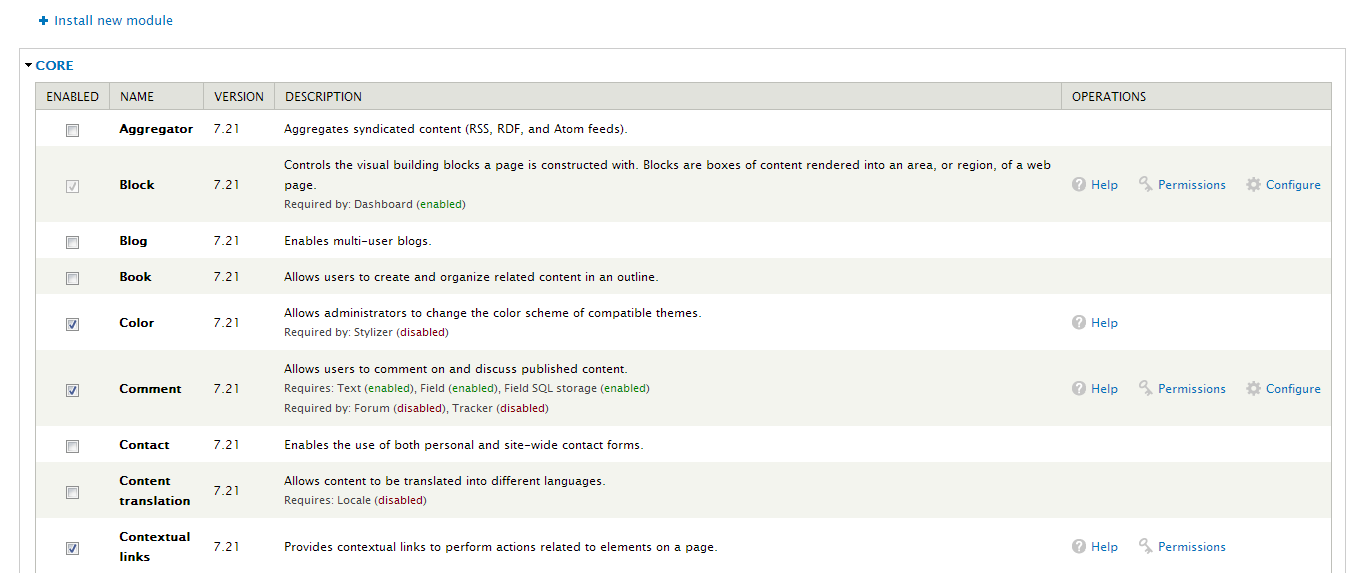
\includegraphics[width=1\textwidth]{fig/drupalOrganizeModules}
\caption{Organisatie van Drupalmodules}
\label{fig:drupalOrganizeModules}
\end{figure}

\subsubsection{Taxonomy}
Taxonomy geeft je de mogelijkheid om eigenschappen en categorie\"{e}n toe te voegen aan je content, zodat bijvoorbeeld een gebruiker content kan filteren uit een grote verzameling. Het biedt dus een manier om je content te organiseren. Een praktijkvoorbeeld is een receptensite, een gebruiker kan dan recepten filteren aan de hand van de eigenschappen van het gerecht (ingredi\"{e}nten, moeilijkheid, ...).

\subsubsection{Users, Roles en Permissions}
Users zijn de gebruikers van jouw website die zich aangemeld hebben. Alle user functionaliteit zoals registreren, inloggen, enz... zit reeds in de Drupal core. Roles geven weer tot welk type een gebruiker hoort. Meerdere gebruikers kunnen dezelfde role hebben, en een gebruiker kan meerdere roles hebben. Met permissions kan je aangeven welke privileges een user met een bepaalde role heeft en dus wat die gebruiker mag en kan doen. Deze permissions worden gekoppeld aan een role zodat alle gebruikers die deze role hebben automatisch de privileges hebben van deze role. Drupal biedt standaard de Administrator role aan die alle privileges heeft.

\subsubsection{Hooks}
Hooks zijn functies die gedefinieerd zijn door de Drupal core. Ze kunnen worden ge\"{i}mplementeerd door elke module. In de Drupal bootstrap zal de Drupal core dan op bepaalde tijdstippen de bijhorende hooks oproepen van elke module die de hook ge\"{i}mplementeerd heeft. Hiervoor wordt een zeer eenvoudig mechanisme gehanteerd. Een module kan zo'n hook defini\"{e}ren door de naam van de hook te laten voorafgaan door de naam van de module die de hook implementeert (zie figuur~\ref{fig:drupalHookExample}).
\begin{figure}[h]
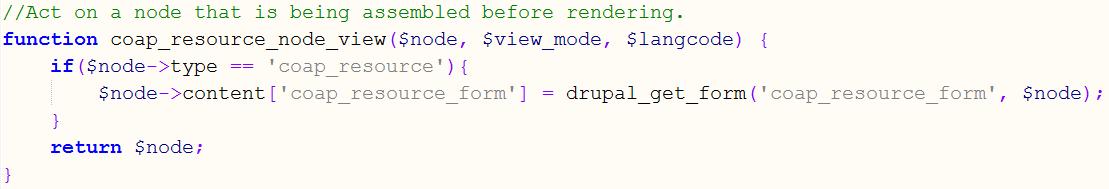
\includegraphics[width=1\textwidth]{fig/drupalHookExample}
\caption{Implementatie van hook\_node\_view door de module coap\_resource}
\label{fig:drupalHookExample}
\end{figure}

\subsubsection{Drupal Core}
De Drupal core is wat je downloadt van de Drupal website. Het vormt de basis en een uitgebreide out-of-the-box functionaliteit, het fungeert eigenlijk als de motor achter een Drupal website. De Drupal Core is zeer uitgebreid en complex, het vormt op zich al voldoende materiaal voor een scriptie, er verder op ingaan zou ons dus te ver leiden.

\subsubsection{Entities}
Een nieuw belangrijk concept in Drupal 7 is entities \cite{entities}. Dit nieuwe concept in combinatie met de Entity API heeft twee positieve effecten. Het eerste effect is dat gebruikers en commentaren dezelfde mogelijkheden krijgen als nodes. In vorige versies van Drupal was het niet mogelijk versies te cre\"{e}eren of velden toe te voegen aan gebruikers of commentaren. Andere voordelen zoals het gebruiken van views in combinatie met gebruikers of commentaren was ook niet mogelijk. Het andere effect is het invoeren van object-ge\"{o}rienteerd programmeren van entities. Vroeger was het nodig specifieke functies van de core te gebruiken om content te bewerken. Een voorbeeld hier van is node\_save() dat nodes opslaat. Deze functie was enkel toepasbaar op een node. Het alternatief bij de Entity API is entity\_save(). Deze functie is niet gelimiteerd tot enkel content of enkel tot gebruikers.
Het is ook mogelijk nieuwe entities te maken, we gaan hier dieper op in in hoofdstuk~\ref{uitbreidingen}.

\subsection{Pagina aanroepen}
Elke keer een webbrowser een Drupal pagina opvraagt, gebeurt er een reeks complexe stappen die als eindresultaat de gerenderde pagina hebben. Indien de pagina niet aanwezig is in de cache, worden deze complexe stappen gegroepeerd in twee delen: de bootstrap en de uitvoering van de page callback. De bootstrap bestaat steeds uit dezelfde reeks van acht verschillende fasen die we verder nader toelichten. Na de bootstrap wordt de page callback uitgevoerd. Indien de pagina wel in de cache aanwezig is, wordt er een subset van de stappen van de bootstrap uitgevoerd. Het hele proces wordt weergegeven in Figuur~\ref{fig:drupalPageRendering}.

\begin{figure}
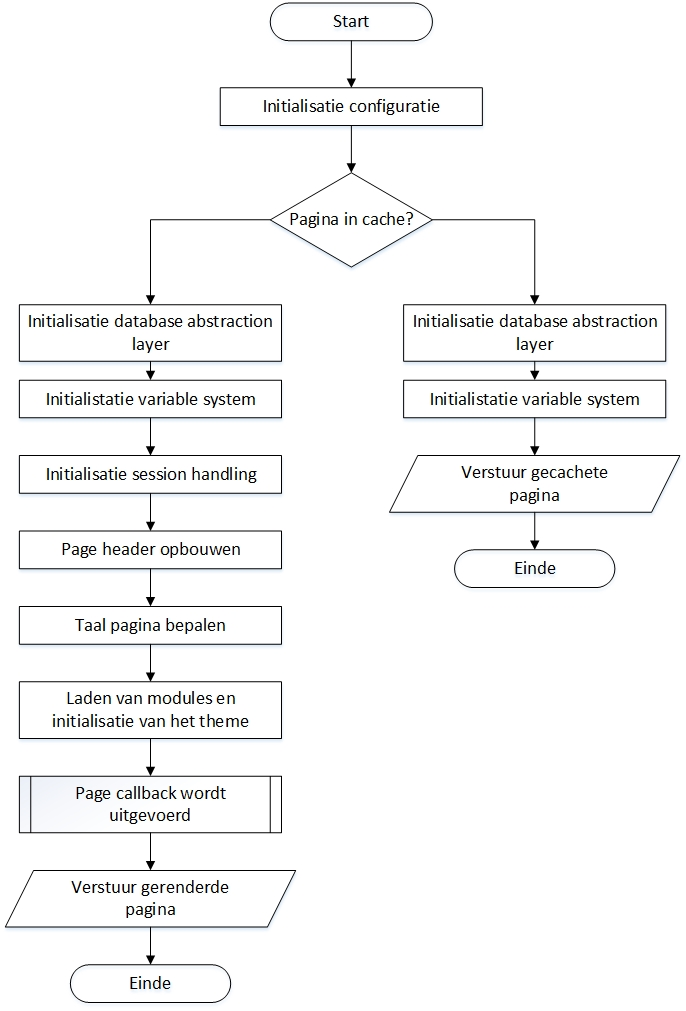
\includegraphics[width=1\textwidth]{fig/drupalPageRendering}
\caption{Pagina renderen in Drupal}
\label{fig:drupalPageRendering}
\end{figure}

\subsubsection{Initialisatie van de configuratie}
Deze fase houdt onder andere in dat globale variabelen worden gezet, zoals de basis URL van de website. Deze configuratie gebeurt aan de hand van een configuratiebestand en aan de omgeving waarin de server zich bevindt.

\subsubsection{Poging tot opvragen van een gecachte pagina}
In deze fase tracht Drupal te vermijden dat de volledige bootstrap moet worden doorlopen. Wanneer de pagina al eens is opgevraagd en deze nog geldig is, wordt deze pagina getoond.

\subsubsection{Initialisatie van de database abstraction layer}
Basisklassen en functies worden ge\"{i}nitialiseerd, maar er worden nog geen verbindingen met de databank opgezet.

\subsubsection{Initialisatie van het Variable System}
In deze fase worden de waarden van variabelen uit de variabelentabel gehaald, die zich in de databank bevindt, en ingevuld bij de juiste naam. Als er modules zijn waarvan hooks moeten worden opgeroepen, worden deze ook ingeladen.

\subsubsection{Initialisatie Session Handling}
In deze fase wordt aan elke user een sessie gekoppeld. Een anonieme user krijgt geen sessie toegewezen tenzij er iets in de sessie moet worden opgeslagen.

\subsubsection{Page Header opbouwen}
De eerste HTTP headers worden opgebouwd, deze worden echter nog niet verstuurd, dit gebeurt pas op het einde van de cyclus. In deze fase vormt zich de eerste mogelijkheid voor modules om functionaliteit in te pluggen in de cyclus van de pagina.

\subsubsection{De taal van de pagina bepalen}
Als de website meerdere talen ondersteunt wordt in deze fase de gekozen taal van de gebruiker bepaald.

\subsubsection{Laden van modules en initialisatie van het theme}
Alle ingeschakelde modules worden ingeladen en het theme wordt ge\"{i}nitialiseerd. Deze fase biedt ook nog de mogelijkheid om variabelen in te stellen die pas later in de request beschikbaar zijn.

\subsubsection{Uitvoeren van page callback}
Drupal bouwt en rendert de pagina.

\newpage

\section{jQuery in Drupal} \label{jQuery}

\begin{wrapfigure}{r}{0.25\textwidth}
\vspace{-40pt}
\hspace{-10pt}
\centering
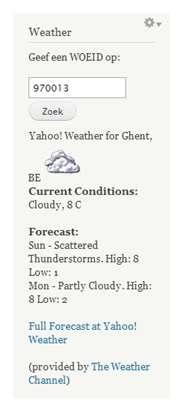
\includegraphics[width=0.3\textwidth]{fig/weermodule}
\vspace{-30pt}
\hspace{-10pt}
\centering
\caption{Weermodule}
\label{fig:weermodule}
%\centering
\vspace{-70pt}
\end{wrapfigure}

In deze paragraaf bekijken we hoe een module (weather\_info) gemaakt werd die het weerbericht ophaalt voor een regio naar keuze, aangegeven door een WOEID. In eerste instantie werd gewerkt met een formulier, maar in een latere fase werd overgestapt op jQuery, wat de gebruikerservaring bevordert.

\subsection{Met een formulier}

In eerste instantie bevatte de module een formulier bestaande uit een textbox als invoer voor de WOEID en een knop om het formulier in te dienen.
Wanneer de gebruiker op de knop klikt, gebeuren volgende stappen:

\begin{itemize}
	\item het formulier wordt ingediend
	\item de pagina wordt opnieuw geladen
	\item de bootstrapcode roept de hook hook\_form\_submit() op door weather\_location\_form\_submit() op te roepen (weather\_location is de naam van het formulier):
	\begin{itemize}
		\item het ingegeven WOEID wordt opgeslagen op serverniveau met de Drupal-functie variable\_set()
	\end{itemize}
	\item de bootstrapcode roept de hook hook\_block\_view op van de weermodule door weather\_info\_block\_view() op te roepen:
	\begin{itemize}
		\item het ingegeven WOEID wordt opgehaald met behulp van de Drupal-functie variable\_get()
		\item er wordt een HTTP-request uitgevoerd naar de Yahoo Weather API met de PHP-functie file\_get\_contents(), dat een URL als parameter verwacht.
		\item het ontvangen xml-bestand wordt in een object gestopt met de PHP-functie SimplexmlElement(), waarna het weerbericht gemakkelijk uit het XML-bestand kan gehaald worden
		\item Het weerbericht wordt toegevoegd aan de inhoud van het block
	\end{itemize}
	\item De pagina wordt in de browser weergegeven met het weerbericht in het block
\end{itemize}

\subsection{Met AJAX in jQuery}

Een pagina zal pas getoond worden wanneer de bootstrap afgelopen is en aangezien de code in de hooks die worden uitgevoerd onderdeel is van de bootstrap, zal de pagina pas getoond worden wanneer de hooks afgelopen zijn. Dit heeft als gevolg dat de gebruiker van de website langer moet wachten op de pagina omdat eerst nog een HTTP-request moet gebeuren om het weerbericht op te halen. Het spreekt voor zich dat dit een zeer nadelig effect is dat moet vermeden worden.\\
Als alternatief hebben we gekozen om een jQuery-event te koppelen aan de submit-knop die het formulier indient. jQuery is namelijk geschreven in JavaScript en JavaScript is een client-side scripting language, wat inhoudt dat deze code wordt uitgevoerd op de machine van de gebruiker en dit nadat de pagina geladen is.\\
Wanneer de gebruiker op de knop klikt, wordt een Asynchronous JavaScript and XML(AJAX)-call\nomenclature{AJAX}{Asynchronous JavaScript and XML} uitgevoerd.
Zoals de naam suggereert, is dit een asynchrone aanroep, wanneer het antwoord aankomt wordt automatisch een opgegeven functie opgeroepen waarin de data kan verwerkt worden. Als gevolg heeft de gebruiker dus geen enkele hinder van het internetverkeer dat noodzakelijk is om het weerbericht op te halen.


\subsection{Problemen}

jQuery laat geen cross-domain AJAX calls toe wegens veiligheidsoverwegingen. Een oplossing hiervoor is een proxy-script in PHP gebruiken.
De AJAX call gebeurt dan naar het proxy script dat zich op de server en dus hetzelfde domein bevindt. Het proxy-script vraagt daar effectief de data op en geeft de uitvoer terug.
De browser wordt dus eigenlijk om de tuin geleid. \cite{crossDomainProblem}
